\documentclass[10pt,aspectratio=169]{beamer}
\usetheme{Execushares}

%\RequirePackage{flashmovie}

\usepackage[algoruled]{algorithm2e}

\renewcommand{\raggedright}{\leftskip=2pt \rightskip=2pt plus 0cm} 


%\usepackage[maxcitenames=2,backend=biber,sorting=ynt]{biblatex}
%\addbibresource{lubric2013.bib}

\newcommand{\citex}[1]{\citeauthor{#1}, \citeyear{#1}}

\usepackage{multirow} %multifilas

\usepackage{booktabs}

\usepackage{multimedia}

\usepackage{bm}

\graphicspath{{figs/}}

\usepackage{color}
\usepackage{amsmath,amsthm,amsfonts}

\newcommand{\hzerooneOm}{{H_0^1(\Omega)}}
\newcommand{\hzerooneom}{{H_0^1(\omega)}}
\newcommand{\honeOm}{{H^1(\Omega)}}
\newcommand{\honeom}{{H^1(\omega)}}
\newcommand{\lpOm}[1]{{L^{#1}(\Omega)}}
\newcommand{\lpom}[1]{{L^{#1}(\omega)}}
\newcommand{\parder}[2]{\frac{\partial #1}{\partial #2}}
\newcommand{\pardertwo}[2]{\frac{\partial^2 #1}{\partial #2^2}}
\newcommand{\parderD}[2]{\frac{\mbox{D} #1}{\mbox{D} #2}}
\newcommand{\parderDtwo}[2]{\frac{\mbox{D}^2 #1}{\mbox{D} {#2}^2}}

\newcommand{\tm}[1]{\textnormal{\scriptsize{#1}}}
\newcommand{\pcc}{p_{\textnormal{\scriptsize{cc}}}}
\newcommand{\pcav}{p_{\textnormal{\scriptsize{cav}}}}
\newcommand{\peq}{p_{\textnormal{{eq}}}}
\newcommand{\Req}{R_{\textnormal{{eq}}}}

\newcommand{\hzero}{H^1_0\left(\Omega\right)}
\newcommand{\hone}{H^1\left(\Omega\right)}
\newcommand{\honedual}{H^{-1}\left(\Omega\right)}
\newcommand{\sobz}[2]{W_0^{#1,#2}\left(\Omega\right)}
\newcommand{\sob}[2]{W^{#1,#2}\left(\Omega\right)}
\newcommand{\cont}{C\left(\bar{\Omega}\right)}
\newcommand{\norm}[2]{\left\lVert#1\right\rVert_{#2}}
\newcommand{\Sp}[1]{\textnormal{Sp}\left(#1\right)}
\newcommand{\Vp}[1]{\textnormal{Vp}\left(#1\right)}

\DeclareMathOperator*{\essinf}{ess\,inf}

\setbeamertemplate{theorems}[numbered]
\title{New models and Numerical Methods in Hydrodynamic Lubrication}
\author{Alfredo Jaramillo}
\date{February 7, 2019}

\newenvironment{nalign}{
	\begin{equation}
	\begin{aligned}
}{
	\end{aligned}
	\end{equation}
	\ignorespacesafterend
}

\newenvironment{nalign*}{
	\begin{equation*}
	\begin{aligned}
}{
	\end{aligned}
	\end{equation*}
	\ignorespacesafterend
}
\usepackage{color}

\setcounter{showSlideNumbers}{1}

\begin{document}
\setcounter{showProgressBar}{0}
\setcounter{showSlideNumbers}{1}

\frame{\titlepage}

\setcounter{showSlideNumbers}{0}
\section{Introduction}
\setcounter{showSlideNumbers}{1}

%==============================================================

\begin{frame}
\frametitle{Lubrication hypothesis}
\vspace*{0.5cm}
\begin{figure}\hspace*{-0.3cm}
	\includegraphics[scale=0.7]{lubscheme_3d.pdf}
\end{figure}
\end{frame}

%==============================================================


\begin{frame}
\frametitle{Layout}
\tableofcontents[hideallsubsections]
\end{frame}

\subsection{Motivation}

%==============================================================
\begin{frame}
\frametitle{The Journal Bearing}
\vspace*{0.7cm}
\begin{figure}
	\centering
	\includegraphics[scale=0.55]{journal_bearing.pdf}
\end{figure}

\end{frame}

%==============================================================

\begin{frame}
\frametitle{The Piston-Ring-Cylinder device}
\vspace*{0.5cm}
\begin{figure}\hspace*{-0.3cm}
	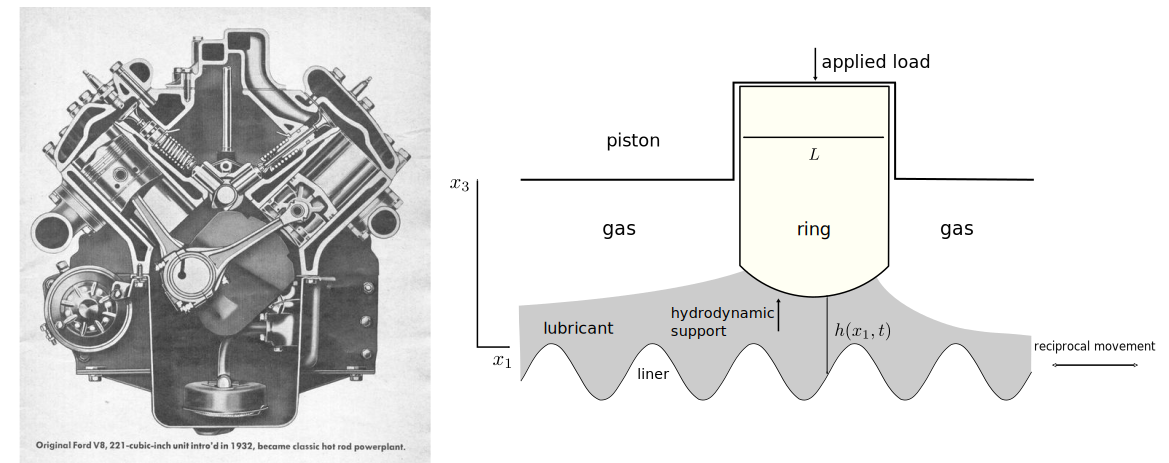
\includegraphics[scale=0.49]{esquema_experimentoF.pdf}
\end{figure}
\end{frame}



%==============================================================

\subsection{Reynolds Equation and cavitation modeling}

%==============================================================

\begin{frame}
\frametitle{The Reynolds Equation}\bigskip
Find the hydrodynamical pressure $p$ such that
\begin{align*}
\nabla \cdot \left( \frac{\rho h^3}{12\,\mu} \nabla p -\frac{\mathbf{U}}{2}\rho h \right) &=\parder{\rho h }{t} &&\text{in } \Omega\subset \mathbb{R}^2~,\\
p&=p_\partial&&\text{on } \partial \Omega~.
\end{align*} 
\begin{itemize}
	\item $h$, $\mathbf{U}$: surfaces' evolution;
	\item $\rho$, $\mu$: fluid' density and viscosity resp.;
	\item $p_\partial\in \mathbb{R}$.
\end{itemize}

\begin{center}
	but cavitation must be considered: $\rho=\rho(p)$
\end{center}
\end{frame}

%==============================================================

\begin{frame}[noframenumbering]
\frametitle{Observation of cavitation in a Journal Bearing}
\vspace*{1.0cm}
\begin{figure}
	\centering
	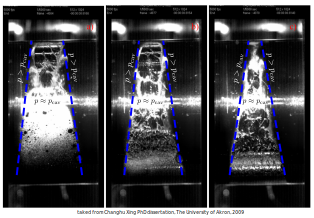
\includegraphics[scale=0.3]{cavitation_journal_bearing.pdf}
\end{figure}
\end{frame}


%==============================================================
\begin{frame}
\frametitle{Cavitation and water treatment}
\vspace*{0.5cm}
\begin{minipage}{\linewidth}
\begin{figure}
	\includegraphics[scale=0.6]{water_treatment.pdf}
\end{figure}
\end{minipage}
\end{frame}

%==============================================================

%\begin{frame}
%\frametitle{Observation of cavitation in a Journal Bearing}
%\vspace*{1.0cm}
%\begin{figure}
%	\centering
%	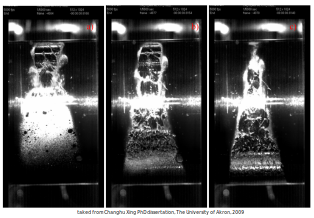
\includegraphics[scale=0.3]{cavitation_journal_bearing0.pdf}
%\end{figure}
%\end{frame}

%==============================================================

\begin{frame}
\frametitle{The Elrod-Adams cavitation model}
\vspace*{1.0cm}
Find $p\geq p_{\text{cav}}$ and $0\leq \theta \leq 1$ such that: $$Q=\frac{h^3}{12\,\mu} \nabla p - \frac{\mathbf{U}}{2}h\theta~,$$ accomplishes (+ b.c.): $$\text{div} \left( Q \right) =\parder{h\theta }{t}\qquad \mbox{and}\qquad p(1-\theta)=0 \qquad \mbox{in }  \Omega~.$$

\begin{figure}
	\centering
	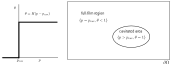
\includegraphics[scale=0.6]{cavitation_omega.pdf}
\end{figure}
\end{frame}

%=============================================================

\setcounter{showSlideNumbers}{0}
\section{Elrod-Adams model: an extension for non-trivial boundary conditions}
\subsection{The separation boundary}
\begin{frame}[noframenumbering]

\tableofcontents[
currentsection,
currentsubsection,
subsectionstyle=show/shaded/hide
]
\end{frame}
\setcounter{showSlideNumbers}{1}

%=============================================================
\begin{frame}
\frametitle{Separation boundary in a Piston-Ring}
\vspace*{1.0cm}
\begin{figure}
	\centering
	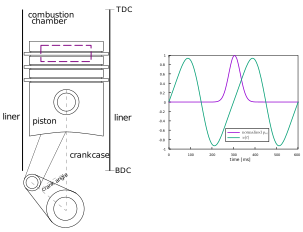
\includegraphics[scale=1.2]{piston-ring-liner.pdf}
\end{figure}
\end{frame}


%=============================================================
\begin{frame}
\frametitle{Separation boundary in a Piston-Ring}
\vspace*{1.0cm}
\begin{figure}
	\centering
	\includegraphics[scale=0.8]{cav_ring1.pdf}
	\caption{\color{ExecusharesGrey}\tiny Author: Dellis, P. 10th International Symposium on Cavitation - CAV2018}
\end{figure}
\end{frame}

%=============================================================
\begin{frame}[noframenumbering]
\frametitle{Separation boundary in a Piston-Ring}
\vspace*{1.0cm}
\begin{figure}
	\centering
	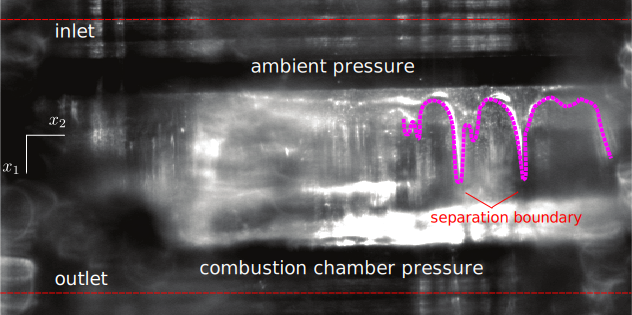
\includegraphics[scale=0.8]{cav_ring2.pdf}
		\caption{\color{ExecusharesGrey}\tiny Adapted from the work of Dellis, P.}
\end{figure}
\end{frame}

%=============================================================
\begin{frame}
\frametitle{Separation boundary in a Piston-Ring}
\vspace*{1.0cm}
\begin{figure}
	\centering
	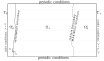
\includegraphics[scale=1.0]{omega_piston_extension_elrod.pdf}
\end{figure}
\end{frame}

\setcounter{showSlideNumbers}{0}
\subsection{Extension of the Elrod-Adams model}
\begin{frame}[noframenumbering]
\tableofcontents[
currentsection,
currentsubsection,
subsectionstyle=show/shaded/hide
]
\end{frame}
\setcounter{showSlideNumbers}{1}

%=============================================================
\begin{frame}
\frametitle{Extending the Elrod-Adams model}
\vspace*{1.0cm}
\begin{minipage}{0.5\linewidth}
Find $p(\textbf{x},t)$ and $\theta(\textbf{x},t)$, $\textbf{x}\in\Omega$ and $t\in[0,t_\textnormal{f}>0]$, such that
\begin{align*}
\nabla\cdot \left( \frac{h^3}{12\,\mu} \nabla p -\frac{\mathbf{U}}{2}h\theta\right) &=\parder{h\theta }{t} &&\text{in } \Omega\\
p&\geq \only<1>{0}
\only<2>{{\color{red}T(\theta)}}&&\text{in } \Omega\\
0\leq \theta &\leq 1&&\text{in } \Omega\\
\only<1>{p(1-\theta)}
\only<2>{(p-{\color{red}T(\theta)})(1-\theta)}&=0 && \text{in } \Omega\\
p &= 0 && \text{on } \Gamma_0\\
p &= \pcc && \text{on } \Gamma_+\\
\theta &= \theta_{\textnormal{in}} && \text{on } \partial\Omega
\end{align*} 
\end{minipage}%
\hspace*{0.3cm}
\begin{minipage}{0.5\linewidth}
\only<2>{
\begin{equation*}
(T\theta)(\mathbf{x})=
\begin{cases}
\pcc(t)  & \text{ if } \mathbf{x}\in \Omega_0^\textnormal{r}\\
0 				& \text{ if } \mathbf{x} \in \Omega_0'\cup \Omega_+
\end{cases},
\end{equation*}
This corresponds to the classical Elrod-Adams model for $T\equiv 0$ and $\pcc=0$.\\

It is possible to prove that this model is ill-posed. An additional condition for the pressure gradient at the separation boundary $\partial \Omega_0^\tm{r}$ is required. Here:

$$\parder{p}{\mathbf{n}}\geq 0\qquad \mbox{in } \Omega_+~.$$}
\end{minipage}
\end{frame}

\subsection{Numerical scheme}
\setcounter{showSlideNumbers}{0}
\begin{frame}[noframenumbering]
\tableofcontents[
currentsection,
currentsubsection,
subsectionstyle=show/shaded/hide
]
\end{frame}
\setcounter{showSlideNumbers}{1}

%=============================================================
\begin{frame}
\frametitle{Discretization}
By means of Finite Volumes one gets the system
\begin{align*}
a^{00}_{i,j}\,p^n_{i,j}+e^{00}_{i,j}\,\theta^n_{i,j} &= C_{i,j}(\bm{p}^n,\bm{\theta}^n)~,\\
p_{i,j}^n&\geq T\left(\bm{\theta}^n\right)_{i,j}~,\\
0\leq \theta_{i,j}^n&\leq 1~,\\
\left(p_{i,j}^n-T\left(\bm{\theta}^n\right)_{i,j}\right)\left(1-\theta_{i,j}^n\right)&=0~.
\end{align*}
For $\pcc\equiv 0$ (thus $T\equiv 0$) one gets a system which well-posedness has been proved in the literature along with an algorithm to solve it (Alt, 1980). 
\end{frame}

%=============================================================
\begin{frame}\frametitle{An extended algorithm}\vspace*{0.7cm}\hspace*{-0.5cm}
	\begin{minipage}[c]{0.6\linewidth}\footnotesize 
		\begin{algorithm}[H]

\Begin{
	initialize(k, $\bm{p}^{n,0}$, $\bm{\theta}^{n,0}$, $\bm{p}^{n,k}$, $\bm{\theta}^{n,k}$)\;
	compute $T(\bm{\theta}^{n,k-1})$\;
	\While{change $>$ tol}{
		\For{$i=1\ldots N_{x_1}$, $j=1\ldots N_{x_2}$}{
			\If{$\left(C_{i,j}-e^{00}_{i,j}\right)/a^{00}_{i,j}\,\geq\, T(\bm{\theta}^{n,k-1})_{i,j}$}
			{$p_{i,j}^{n,k} \leftarrow (C_{i,j}-e^{00}_{i,j})/a^{00}_{i,j}$\;
				$\theta_{i,j}^{n,k}\leftarrow 1$\;
				\Else{
					$\theta_{i,j}^{n,k}\leftarrow(C_{i,j}-a^{00}_{i,j}\, T(\bm{\theta}^{n,k-1})_{i,j})/e^{00}_{i,j}$\;
					$p_{i,j}^{n,k} \leftarrow T(\bm{\theta}^{n,k-1})_{i,j}$\;
				}
			}
		}
		\emph{change}$\leftarrow\|\bm{p}^{n,k}-\bm{p}^{n,k-1}\|+\|\bm{\theta}^{n,k}-\bm{\theta}^{n,k-1}\|$\;
		update variables ($k\leftarrow k+1$)\;
	}
}
		\end{algorithm}
	\end{minipage}
	\begin{minipage}{0.35\linewidth}
		 \begin{figure}
		 	\centering
		 	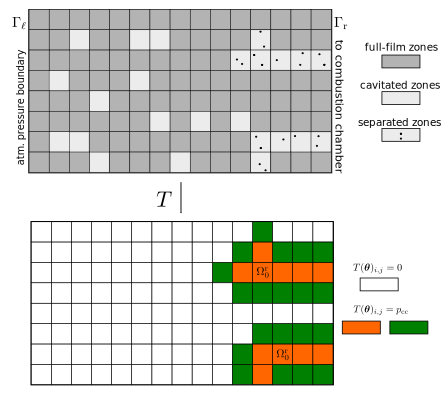
\includegraphics[scale=0.55]{operator_T_discrete}
		 \end{figure}
\end{minipage}
\end{frame}


\subsection{Numerical results}
\setcounter{showSlideNumbers}{0}
\begin{frame}[noframenumbering]
\tableofcontents[
currentsection,
currentsubsection,
subsectionstyle=show/shaded/hide
]
\end{frame}
\setcounter{showSlideNumbers}{1}

%=============================================================
\begin{frame}
\frametitle{Numerical results: Blow-by}
\vspace*{1.0cm}
\begin{minipage}{0.5\textwidth}
	\begin{figure}
		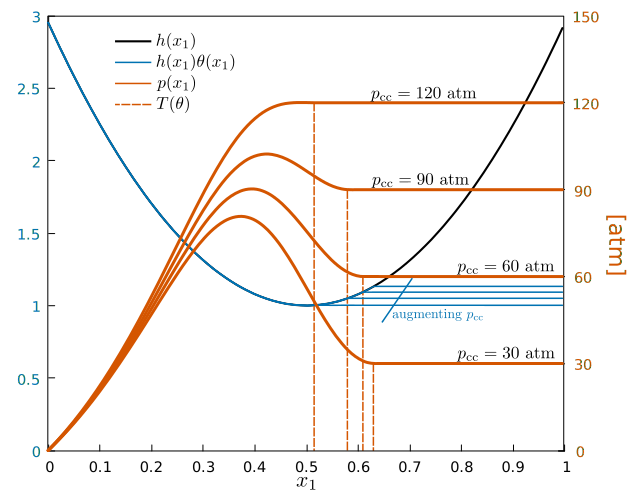
\includegraphics[scale=0.3]{stationary_cases}
	\end{figure}
\end{minipage}%
\begin{minipage}{0.5\textwidth}
	\begin{figure}
		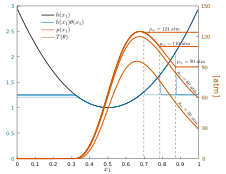
\includegraphics[scale=0.3]{stationary_cases2}
	\end{figure}
\end{minipage}
\end{frame}

%=============================================================
\begin{frame}
\frametitle{Numerical results: A textured ring}\vspace*{0.5cm}
\begin{center}
\begin{minipage}{0.9\textwidth}
	\centering 
	\movie[loop,showcontrols]{\includegraphics[width=\textwidth]{videos/02.png}}{videos/comparison_reynolds.ogv}
\end{minipage}
\end{center}

\end{frame}

%=============================================================
\begin{frame}
\frametitle{Numerical results: A textured ring}\vspace*{0.5cm}
\begin{minipage}{0.45\linewidth}
\begin{figure}
	\centering
	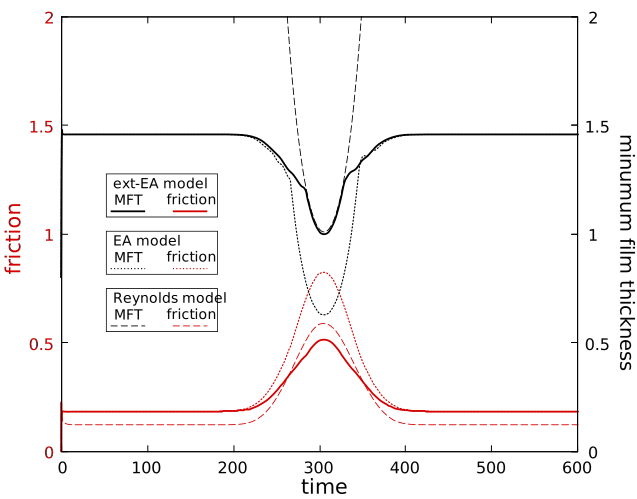
\includegraphics[scale=0.35]{friction_hmin_time}
\end{figure}
\end{minipage}
%
\begin{minipage}{0.45\linewidth}
\begin{table}\hspace*{2cm}
		\begin{tabular}{ccc}
			\toprule
			& EA/eEA & Reynolds/eEA\\
			\midrule
			$\frac{|\bar{f}-\bar{f}^*|}{|\bar{f}^*|}$ & 17\% & 25\% \\
			\bottomrule
	\end{tabular}
\end{table}
\end{minipage}
\end{frame}

%=============================================================
\begin{frame}
\frametitle{Numerical results: A ring with wear}
\vspace*{1.0cm}
\begin{figure}
	\centering
	\includegraphics[scale=0.55]{ring_wear}
\end{figure}

\begin{table}\centering {\small
		\begin{tabular}{cccccccccc}
			\toprule
			\multirow{2}{*}{} &
			
			\multicolumn{7}{c}{$\Delta h$ (microns)} \\
			& 0.5 & 1.0& 1.5& 2.0 & 2.5& 3.0 & 3.5 &3.91& 4.0-8.0\\
			\midrule
			$\delta^\tm{max}$ (microns) & 0.025 &0.035 & 0.040 & 0.045 & 0.050 & 0.055 & 0.025& 0.005&0\\
			\bottomrule
	\end{tabular}}
	\caption{Minimum value of $\delta$ for which the simulations fail for every $\delta\geq \delta_\tm{max}$.}\label{tab:hmax}
\end{table}
\end{frame}

%=============================================================

\setcounter{showSlideNumbers}{0}
\section{Reynolds-Rayleigh-Plesset model: well-posedness}

\begin{frame}[noframenumbering]
\tableofcontents[
currentsection,
currentsubsection,
subsectionstyle=show/shaded/hide
]
\end{frame}
\setcounter{showSlideNumbers}{1}

%==============================================================
\begin{frame}
\frametitle{Motivation}
\begin{itemize}
	\item The Reynolds-Rayleigh-Plesset coupled system captures the physics of gaseous cavitation.
	\item This type of models are used in several numerical works to model cavitation along a flow equation (e.g., Navier-Stokes/Reynolds equations in the Software FLUENT).

\end{itemize}
\end{frame}

\subsection{The Reynolds-Rayleigh-Plesset coupling}

%==============================================================
\begin{frame}
\frametitle{The Rayleigh-Plesset equation}
\vspace*{1.0cm}
\hspace*{-0.5cm}
\begin{minipage}{0.4\textwidth}
Knowing $p$ \emph{far away from} the bubble of radius $R$
\begin{equation*}
\overbrace{\rho_\ell\left(\frac{3}{2}\dot{R}^2+R\ddot{R}\right)}^{\text{inertial terms}}=\overbrace{p_\textnormal{b}-p-\frac{2\sigma}{R}}^{\text{Young-Laplace eq.}}\overbrace{-\left(\mu_\ell+\frac{\kappa^s}{R}\right)\frac{4\dot{R}}{R}}^{\text{viscuous terms}}
\end{equation*}
\end{minipage}%
\hspace*{0.8cm}
\begin{minipage}{0.5\textwidth}
\begin{figure}[h]
	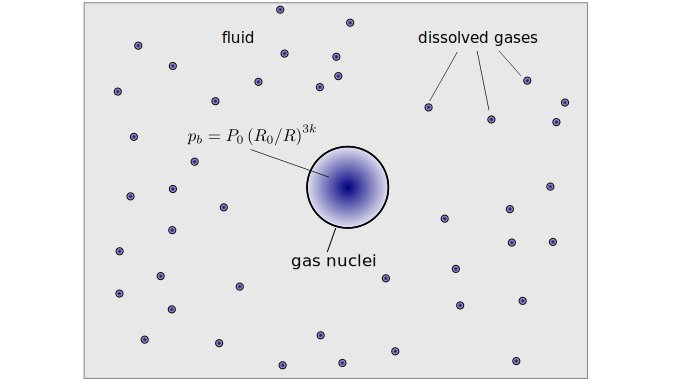
\includegraphics[scale=0.55]{gaseous_cavitation.pdf}
\end{figure}
\end{minipage}
\begin{center}
So we have the relation $p\longrightarrow R$
\end{center}
\end{frame}

%==============================================================
\begin{frame}
\frametitle{A model for the cavitation pressure}
\begin{minipage}{0.3\textwidth}
In the equilibrium:
$$\peq(\Req)=p_\textnormal{b}(\Req)-\frac{2\sigma}{\Req}~.$$
The minimum of this curve is called \emph{cavitation pressure}.\\

Notice that in the \emph{stable branch} one has $$\peq'(\Req)<0~.$$
\end{minipage}%
\hspace*{0.5cm}
\begin{minipage}{0.5\textwidth}\vspace*{1.0cm}
	\begin{figure}
	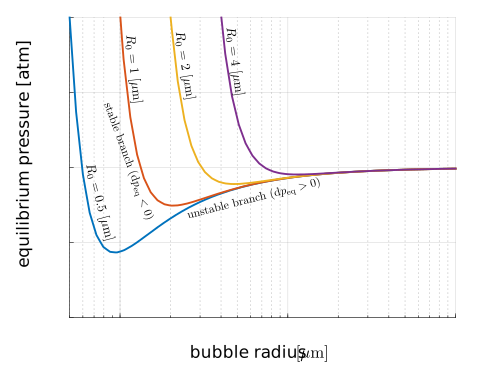
\includegraphics[scale=0.7]{peq_req}
	\caption{Equilibrium states $(\peq^*,\Req^*)$ for several values of $R_0$ and $P_0=1\,\mbox{[atm]}$.}
\end{figure}
\end{minipage}
\end{frame}

%==============================================================
\begin{frame}
\frametitle{The Reynolds-Rayleigh-Plesset coupling}
Assuming a mono-disperse bubbles distribution, find $p(\mathbf{x},t)$ and $R(\mathbf{x},t)>0$ such that:
\begin{align*}
\nabla\cdot\left(\frac{\rho\left(\alpha\right) h^3}{12\mu\left(\alpha\right) }\nabla p-\frac{\mathbf{U}}{2}\rho\left(\alpha\right) h \right)&=\parder{\rho\left(\alpha\right) h}{t}&&\alpha \longrightarrow p~,\\
\rho_\ell\left(\frac{3}{2}\left(\parderD{R}{t}\right)^2+R\parderDtwo{R}{t}\right)&=p_b-\frac{2\sigma}{R}-p-\left(\mu_\ell+\frac{\kappa^s}{R}\right)\frac{4}{R}\parderD{R}{t}&&p\longrightarrow R~,\\
\alpha(R)&=\frac{\mbox{volume of gas}}{\mbox{volume of gas and liquid}}&&R\longrightarrow \alpha~.
\end{align*}
along suitable initial conditions.
\begin{center}
	Is this evolution problem  well-posed?\\
	Existence - uniqueness - stability
\end{center}
\end{frame} 

%==============================================================

\begin{frame}
\frametitle{The abstract problem: full RP equation}
Disregarding the convection of the field $R$, find $p(\mathbf{x},t)$ and $R(\mathbf{x},t)>0$ such that:
\begin{equation}
\underbrace{\frac{3}{2}\frac{1}{R}\left(\parder{R}{t}\right)^2+\frac{\partial^2 R}{\partial t^2}}_{\textnormal{inertial terms}}=\frac{f_1\left(R\right)-p}{R}-\parder{R}{t}f_2\left(R\right)~,\label{eq:abstract-rp1}
\end{equation}
and
\begin{align}
\begin{split}
\nabla_x\cdot \left(f_3\left(R\right) h^3\,\nabla p\right)&=\nabla_x\cdot \left(f_4\left(R\right)\mathbf{U}\,h\,\right)+h\,f_5\left(R\right)\parder{R}{t},\\
p&=0 \qquad\mbox{on } \partial \Omega~.
\end{split}
\label{eq:abstract-reynolds1}
\end{align}

\end{frame} 

%==============================================================

\begin{frame}
\frametitle{Well-posedness of the coupled system}
\begin{equation*}
	f_1\left(R\right)=p_b-\frac{2\sigma}{R}-p_\partial~,
\end{equation*}
\begin{align*}
f_2\left(R\right)&=4\left(\frac{\mu_\ell+\kappa^s/R}{R^2}\right)~,&f_3\left(R\right)&=\frac{1}{12}\frac{(1-\alpha\left(R\right))\rho_\ell+\alpha\left(R\right)\rho_g}{(1-\alpha\left(R\right))\mu_\ell+\alpha\left(R\right)\mu_g}~,\\ f_4\left(R\right)&=\frac{1}{2}\left[\rho_\ell+\alpha\left(R\right)\left(\rho_g-\rho_\ell\right)\right]~,&f_5\left(R\right)&=f_4'\left(\alpha\left(R\right)\right)\,\alpha'\left(R\right)~.
\end{align*}

\begin{itemize}
	\item[H1:] $f_1\in C^2\left(\mathbb{R}^+_*;\mathbb{R}\right)$, $${\color{red}\exists \bar{R},\delta_1\in\mathbb{R}^+_*~\text{s.t.}~f_1\left(\bar{R}\right)=0~\text{and}~f'_1\left(R\right)<0\, \forall R \in [\bar{R}-\delta_1,\bar{R}+\delta_1]}$$
\end{itemize}
Additional hypotheses on the $f_i$ functions are made.
\end{frame} 

%==============================================================

%\begin{frame}
%\frametitle{Well-posedness of the coupled system}
%\begin{itemize}
%	\item[H1:] $f_1\in C^2\left(\mathbb{R}^+_*;\mathbb{R}\right)$, $${\color{red}\exists \bar{R},\delta_1\in\mathbb{R}^+_*~\text{s.t.}~f_1\left(\bar{R}\right)=0~\text{and}~f'_1\left(R\right)<0\, \forall R \in [\bar{R}-\delta_1,\bar{R}+\delta_1];}$$
%	\item[H2:] $f_2\in C^2\left(\mathbb{R}_*^+;\mathbb{R}^+_*\right)$;
%	\item[H3:] $f_3\in C^2\left(\mathbb{R}_*^+;\mathbb{R}\right)$ and $\exists m_3,M_3>0$ such that $m_3\leq f_3\left(r\right)\leq M_3$ $\forall r\in \mathbb{R}^+$;
%	\item[H4:] $f_4\in C^2\left(\mathbb{R}_*^+;\mathbb{R}^+\right)$, $f_4'\left(r\right)<0$ $\forall r>0$;
%	\item[H5:] $f_5\in C^2\left(\mathbb{R}_*^+;\mathbb{R}^-_*\right)$;
%	\item[H6:] $h \in B_{m_0,M_0}$ for $0<m_0<M_0$ constants. Denoting $h_0=\underset{\Omega}{\essinf{\,h}}$.
%\end{itemize}
%With $B_{\alpha,\beta	}=\left\{w\in L^\infty\left(\Omega\right):\alpha \leq w \leq \beta\mbox{ a.e. on } \Omega \right\}.$
%\end{frame} 

%==============================================================

\subsection{Local existence in time}
\setcounter{showSlideNumbers}{0}
\begin{frame}[noframenumbering]
\tableofcontents[
currentsection,
currentsubsection,
subsectionstyle=show/shaded/hide
]
\end{frame}
\setcounter{showSlideNumbers}{1}

%==============================================================

\begin{frame}
\frametitle{The abstract problem: full RP equation}\vspace*{0.5cm}
Find $p(\mathbf{x},t)$ and $R(\mathbf{x},t)>0$ such that:
\begin{equation*}
\frac{3}{2}\frac{1}{R}\left(\parder{R}{t}\right)^2+\frac{\partial^2 R}{\partial t^2}=\frac{f_1\left(R\right)-{\color{red}p}}{R}-\parder{R}{t}f_2\left(R\right)~,
\end{equation*}
and
\begin{align*}
\begin{split}
\nabla_x\cdot \left(f_3\left(R\right) h^3\,\nabla p\right)&=\nabla_x\cdot \left(f_4\left(R\right)\mathbf{U}\,h\,\right)+h\,f_5\left(R\right)\parder{R}{t}~,\\
p&=0 \qquad\mbox{on } \partial \Omega~.
\end{split}
\end{align*}

Along suitable i.c. for $R$ and $\parder{R}{t}$. In order to use the Cauchy-Lipschitz Theorem, we write
\begin{center}
 {\color{red}$p=A\left(R,\parder{R}{t}\right)$} ,
\end{center}
by means of the Reynolds equation. The regularity of the mapping $A$ comes from the Lax-Milgram Theorem and a Sobolev Embedding (Adams, 1975).
\end{frame} 

%==============================================================

\begin{frame}\frametitle{Local existence in time: including inertia}
Then, the problem \eqref{eq:abstract-rp1}-\eqref{eq:abstract-reynolds1} can be rewritten as
\begin{equation}
\begin{split}
\frac{d\tilde{R}}{dt}&=F(\tilde{R})~,\\
\tilde{R}(0)&=\tilde{R}_0~,
\end{split}\label{eq:problem-rewritten}
\end{equation}
where $\tilde{R}=\left(R_1,R_2\right)=\left(R,\parder{R}{t}\right)$, $\tilde{R}_0=(r_1,r_2)\in Q\times \cont$ and $F:Q\times \cont\mapsto \left(\cont\right)^2$ with
\begin{equation}
F(R_1,R_2)=\left(
R_2,~-\frac{3}{2}\frac{R_2^2}{R_1}-R_2f_2\left(R_1\right)+\frac{f_1\left(R_1\right)-A\left(R_1,R_2\right)}{R_1}\right)~.
\end{equation}
Thus, the Cauchy-Lipschitz Theorem implies the local existence result:
\begin{theorem}There exists $T>0$ such that the  problem \eqref{eq:problem-rewritten} has a unique solution in $C^3\left([0,T];Q\times \cont\right)$.
\end{theorem}
\end{frame}

%==============================================================
\begin{frame}
\frametitle{Local existence in time: without inertial terms}
\vspace*{0.6cm}
\begin{equation}
\parder{R}{t}=\frac{f_1\left(R\right)-A\left(R,\parder{R}{t}\right)}{R\,f_2\left(R\right)}=\Pi\left(R,\parder{R}{t}\right)\pause=G(R)~,\label{eq:abstract-rp-inertialess}
\end{equation}
by means of the Fredholm Alternative Theorem one proves that there exists a unique $G\left(R\right)\in \cont$ such that $G\left(R\right)=\Pi\left(R,G\left(R\right)\right),$ and the mapping $G$ is of class $C^2$.
\begin{theorem}There exists $T>0$ such that  problem \eqref{eq:abstract-reynolds1}-\eqref{eq:abstract-rp-inertialess} with i.c. $R\left(\cdot,0\right)=r_1$ in $\Omega$ has a unique solution in $C^3\left([0,T];Q\right)$.
\end{theorem}
The result follows directly from applying the Cauchy-Lipschitz Theorem to the equivalent evolution problem
\begin{equation}
\parder{R}{t}=G(R)~,\label{eq:ev-problem-G}
\end{equation}
along the initial condition written above.
\end{frame} 


%==============================================================

\subsection{Stationary solutions: existence and stability}
\setcounter{showSlideNumbers}{0}
\begin{frame}[noframenumbering]
\tableofcontents[
currentsection,
currentsubsection,
subsectionstyle=show/shaded/hide
]
\end{frame}
\setcounter{showSlideNumbers}{1}

%==============================================================

\begin{frame}
\frametitle{The abstract problem: full RP equation}
Find $p(\mathbf{x},t)$ and $R(\mathbf{x},t)>0$ such that:
\begin{equation*}
\frac{3}{2}\frac{1}{R}\left(\parder{R}{t}\right)^2+\frac{\partial^2 R}{\partial t^2}=\frac{f_1\left(R\right)-p}{R}-\parder{R}{t}f_2\left(R\right)~,
\end{equation*}
and
\begin{align*}
\begin{split}
\nabla_x\cdot \left(f_3\left(R\right) h^3\,\nabla p\right)&=\nabla_x\cdot \left(f_4\left(R\right)\mathbf{U}\,h\,\right)+h\,f_5\left(R\right)\parder{R}{t}~,\\
p&=0 \qquad\mbox{on } \partial \Omega~.
\end{split}
\end{align*}
Along suitable i.c. for $R$ and $\parder{R}{t}$.
\end{frame} 

%==============================================================

\begin{frame}
\frametitle{The stationary problem}

Observe that a stationary solution $(R_s,p_s)$ of problem \eqref{eq:abstract-rp1}-\eqref{eq:abstract-reynolds1} satisfies
\begin{equation*}
p_s=f_1\left(R_s\right)~.
\end{equation*}
Writing $h=h_0+h^+$ with $h_0=\underset{\Omega}{\essinf{\,h}}$, $(R_s,p_s)$ is solution of the system
\begin{nalign}
	\nabla\cdot \left(\left(h_0+h^+\right)^3f_3\left(R_s\right)\nabla p_s\right)&=\nabla\cdot\left(\mathbf{U}\left(h_0+h^+\right)f_4\left(R_s\right)\right)&&\textnormal{ in } \Omega,\\
	p_s&=f_1\left(R_s\right)&&\textnormal{ in } \Omega~,\\
	R_s&>0&&\textnormal{ in } \Omega~,\\
	p_s&=0&&\textnormal{ on }\partial \Omega~.
	\label{eq:problem-stationary}
\end{nalign}
Observe that if $\mathbf{U}=0$ or $h^+=0$ then $\left(R_s,p_s\right)=\left(\bar{R},0\right)$ is solution of \eqref{eq:problem-stationary}.


\end{frame} 

\begin{frame}
\frametitle{The stationary problem}

\begin{figure}[h]
	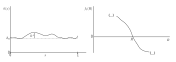
\includegraphics[scale=0.85]{drawing_h_f1.pdf}
\end{figure}

\end{frame} 

%==============================================================

\begin{frame}
\frametitle{Stationary solutions: existence}
\begin{theorem}\label{theo:existence_U_fix}
	Fix $\mathbf{U}\in\mathbb{R}^2$ and $h_0>0$. Then there exists $\epsilon\left(\mathbf{U}\right)>0$ such that the problem \eqref{eq:problem-stationary} has a unique solution $\left(R_s,p_s\right)$ with $R_s>0$ whenever $\norm{h^+}{\infty}<\epsilon(\mathbf{U})$.\\ {\color{red}Moreover, the solution $\left(R_s,p_s\right)$ depends continuously on $h^+$}.
\end{theorem}
\begin{theorem}\label{theo:existence_h_fix}
	Fix $h\in B_{m_0,M_0}$, $0<m_0<M_0$. Then there exists $\epsilon\left(h\right)>0$ such that the problem \eqref{eq:problem-stationary} has a unique solution $\left(R_s,p_s\right)$ with $R_s>0$ whenever $\norm{\mathbf{U}}{}<\epsilon\left(h\right)$.\\  {\color{red}Moreover, the solution $\left(R_s,p_s\right)$ depends continuously on $\mathbf{U}$}.
\end{theorem}
\bigskip

Both results follow from the fact that for $\mathbf{U}=0$ or $h^+=0$ there exists a trivial solution ($p\equiv0$) and the Implicit Function Theorem.
\end{frame} 

%==============================================================
%\begin{frame}
%\frametitle{Proof of Theorem \ref{theo:existence_U_fix}, $U$ fixed}
%\vspace*{0.6cm}
%Since $\nabla p_s=f_1'\left(R_s\right)\nabla R_s$ the problem \eqref{eq:problem-stationary} can be written in function of $\xi$ as
%\begin{nalign}
%	-\nabla\cdot \left(\left(h^++h_0\right)^3a_0\left(\xi\right)\nabla\,\xi\right)&=\nabla\cdot \left(U h^+\,b_0(\xi)\right)+\nabla\cdot \left(Uh_0\,b_0(\xi)\right)&&\textnormal{ in }\Omega,\\
%	\xi&>-\bar{R}&&\textnormal{ in }\Omega,\\
%	\xi&=0&&\textnormal{ on } \partial \Omega,
%	\label{eq:problem-stationary-change}
%\end{nalign}
%where $a_0\left(\xi\right)=-f_3\left(\bar{R}+\xi\right)f_1'\left(\bar{R}+\xi\right)$, and $b_0(\xi)=f_4\left(\bar{R}+\xi\right)$. We introduce the open set
%$$W=\left\{\xi\in W_0^{1,q}\left(\Omega\right):\xi >-\bar{R}\textnormal{ a.e. on } \Omega\right\},$$
%and the application $\phi:W\times L^\infty\left(\Omega\right)\longmapsto W^{-1,q}$:
%\begin{equation}
%\phi(\xi,\delta) =  \nabla\cdot \left(\left(\delta+h_0\right)^3a_0\left(\xi\right)\nabla\,\xi\right)+\nabla\cdot \left(U\delta\,b_0(\xi)\right)+\nabla\cdot \left(Uh_0\,b_0(\xi)\right),
%\end{equation}
%since $\phi(0,0)=0$ and $\partial_\xi\phi(0,0)$ is invertible, the Implicit Function Theorem implies that there exists $\xi=\xi\left(\delta\right)\Leftrightarrow R_s=R_s\left(h^+\right)$ {\color{red}smooth}.
%\end{frame}

%==============================================================

\begin{frame}
\frametitle{Stability of stationary solutions}
\begin{figure}
	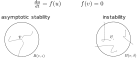
\includegraphics[scale=0.85]{stability.pdf}
\end{figure}
\end{frame}

%==============================================================

\begin{frame}
\frametitle{Stability with inertial terms}
\vspace*{0.5cm}
\begin{equation}
\begin{split}
\frac{d\tilde{R}}{dt}&=F(\tilde{R})~,\\
\tilde{R}(0)&=\tilde{R}_0~,
\end{split}
\end{equation}
where $\tilde{R}_0=\begin{pmatrix}
{r}_1\\ {r}_2
\end{pmatrix}\in Q$ and $F:Q\times \cont\mapsto \left(\cont\right)^2$ with
\begin{equation}
F(R_1,R_2)=\left(
R_2,~-\frac{3}{2}\frac{R_2^2}{R_1}-R_2f_2\left(R_1\right)+\frac{f_1\left(R_1\right)-A\left(R_1,R_2\right)}{R_1}\right)~.
\end{equation}
We denote by $\mathcal{L}_F$ the Fréchet derivative of $F$ at $\left(R_1,R_2\right)=\left(R_s,0\right)$, i.e.,
\begin{equation}
\begin{array}{cccl}
\mathcal{L}_F:&\left(\cont\right)^2&\longmapsto& \left(\cont\right)^2\\
&(S_1,S_2)& \longmapsto & \textnormal{D}F\left(R_s,0\right)\left(S_1,S_2\right)~.\label{eq:jacobian_inertia}
\end{array}
\end{equation} 
It is shown that, for some particular cases, the spectrum of $\mathcal{L}_F$ is such that $$\mbox{Re}\left(\lambda\right)<0\qquad \forall \lambda\in \Sp{\mathcal{L}_F}~.$$
\end{frame}



%==============================================================

\begin{frame}
\frametitle{Stability with inertial terms}\vspace*{0.5cm}
For $h^+=0$ or $\mathbf{U}=0$ one has
\begin{equation}\label{eq:L_F}
\mathcal{L}_F\left(S_1,S_2\right)=B\begin{pmatrix}
S_1\\S_2
\end{pmatrix}-b_r\begin{pmatrix}
0\\\pi_1\left(S_1\right)+\pi_2\left(S_2\right)
\end{pmatrix},
\end{equation}
where $B=\begin{pmatrix}0&1\\-b_1&-b_2
\end{pmatrix}$, $\pi_1(S_1)$ is the solution of:
\begin{nalign}
	-b_3\nabla\cdot \left(h^3 \,\nabla \pi_1\left(S_1\right)\right)&=b_4\nabla\cdot \left(\mathbf{U}\,hS_1\right)&&\textnormal{ in }  \Omega~,\\
	\pi_1\left(S_1\right)&=0 &&\textnormal{ on } \partial \Omega~,
	\label{eq:pi1-triv-case}
\end{nalign}
and $\pi_2(S_1)$ is the solution of:
\begin{nalign}
	-\nabla\cdot \left(h^3f_3\left(R_s\right) \,\nabla \pi_2\left(S_2\right)\right)&=-hf_5\left(R_s\right)S_2&&\textnormal{ in }  \Omega~,\\
	\pi_2\left(S_2\right)&=0 &&\textnormal{ on } \partial \Omega~.
	\label{eq:def:pi2}
\end{nalign}
Denote by $\{\lambda_1^B,\lambda_2^B\}$ the set of eigenvalues of $B$ and notice that $\mbox{Re}\left(\lambda_1^B\right)<0$ and $\mbox{Re}\left(\lambda_2^B\right)<0$.
\end{frame}

%==============================================================

\begin{frame}
\frametitle{Stability with inertial terms}
\vspace*{0.5cm}
\begin{lemma}\label{lemma:spec-L_F}
	Let $h^+=0$ or $\mathbf{U}=0$. Then
	\begin{equation}
	\Sp{\mathcal{L}_F}\subset \Vp{\mathcal{L}_F}\cup \{\lambda_1^B,\lambda_2^B\}.
	\end{equation}
	Moreover if $\lambda\in \Vp{\mathcal{L}_F}\setminus\{\lambda_1^B,\lambda_2^B\}$ with associated eigenfunction $\left(S_1,S_2\right)\in\cont^2$ then $\left(S_1,S_2\right)\in\hzero^2$, $S_2=\lambda S_1$ and $S_1$ is solution of the problem
	\begin{align*}
	\frac{b_3}{b_r}\xi\left(\lambda\right)\nabla\cdot\left(h^3\nabla S_1\right)&=b_4\, \mathbf{U}\cdot\nabla\left(hS_1\right)+\lambda\, b_5 h\, S_1 && \textnormal{in }\Omega,\\
	S_1&=0&&\textnormal{on }\partial\Omega,
	\end{align*}
	where $\xi\left(\lambda\right)=\lambda^2+b_2\lambda+b_1$ with roots $\{\lambda_1^B,\lambda_2^B\}$.
\end{lemma}

\end{frame}

%==============================================================

\begin{frame}
\frametitle{Stability with inertial terms}
\begin{theorem}\label{theo:stabilite-avec-inertie-h-fixe} Let $h\in B_{m_0,M_0}$, $0<m_0<M_0$ (as in Theorem \ref{theo:existence_h_fix}). Then there exists $\epsilon\left(h\right)>0$ s.t. if $\norm{\mathbf{U}}{\infty}<\epsilon$ the solution $\left(R_s,p_s\right)$ of problem \eqref{eq:problem-stationary} is asymptotically stable for the evolution problem \eqref{eq:problem-rewritten}.
\end{theorem}\bigskip
\textbf{Step 1}: Take $\mathbf{U}=0$. Based in the previous Lemma: it is enough to study $\Vp{\mathcal{L}_F}$, and it is possible to prove that  $\mbox{Re}\left(\lambda\right)<0$ $\forall \lambda \in \Vp{\mathcal{L}_F}$.\\ \bigskip
\textbf{Step 2}: From Theorem \ref{theo:existence_h_fix} the mapping $\mathbf{U}\mapsto R_s\left(\mathbf{U}\right)$ is continuous in a neighborhood $V_1\ni 0$ in $\mathbb{R}^2$, thus if $\mathbf{U}\rightarrow 0$ in $\mathbb{R}^2$ then $\norm{\textnormal{D}F\left(R_s\left(\mathbf{U}\right),0\right)-\textnormal{D}F\left(\bar{R},0\right)}{}\rightarrow 0$ in the space of linear continuous operators from $\cont^2$ into itself. This, plus the continuity of the spectrum give us the result.
\end{frame}

%==============================================================

\begin{frame}
\frametitle{Stability with inertial terms}
\begin{theorem}\label{theo:instabilite-avec-inertie-U-fixe} Set $h^+=0$ and consider the one-dimensional case ($N=1$). Then there exists $M>0$ such that if $\norm{\mathbf{U}}{\infty}>M$ the solution $\left(R_s,p_s\right)$ of problem \eqref{eq:problem-stationary} is asymptotically unstable for the evolution problem \eqref{eq:problem-rewritten}.
\end{theorem}\bigskip
It is shown that there exists $\lambda\in \Vp{\mathcal{L}_F}$ such that $\mbox{Re}(\lambda)>0$ for $\mathbf{U}$ big enough.
\end{frame}

%==============================================================

\begin{frame}\frametitle{Stability without inertial terms}
Recalling the evolution problem
\begin{equation}
\parder{R}{t}=G(R)=\Pi\left(R,G\left(R\right)\right)~,
\end{equation}
with i.c. $R\left(\cdot,0\right)=r_1$ in $\Omega$. We denote the derivative
\begin{equation}
\begin{array}{cccl}
\mathcal{L}_G:&\cont&\longmapsto& \cont\\
&w& \longmapsto & \textnormal{D}\,G\left(R_s\right)\left(w\right)~.\label{eq:def-L_G}
\end{array}
\end{equation} 
\bigskip

Notice that the existence theorems (\ref{theo:existence_U_fix}) and (\ref{theo:existence_h_fix}) for solutions of the stationary problem are still valid when disregarding the inertial terms.
\end{frame}

%==============================================================

\begin{frame}\frametitle{Stability without inertial terms}
\begin{theorem} \label{theo:stability-sans-inertie-h-fix}
	Fix $h\in B_{m_0,M_0}$, $0<m_0<M_0$. Then there exists $\epsilon>0$ s.t. if $\norm{\mathbf{U}}{}<\epsilon$ then the solution $\left(R_s,p_s\right)$ of problem \eqref{eq:problem-stationary} is asymptotically stable for the evolution problem \eqref{eq:abstract-reynolds1}-\eqref{eq:abstract-rp-inertialess} along the i.c. $R\left(\cdot,0\right)=r_1$ in $\Omega$
\end{theorem}
\begin{theorem}\label{theo:stability-sans-inertie-U-fixe} For every $U\in \mathbb{R}^2$ there exists $\epsilon=\epsilon\left(\mathbf{U}\right)>0$ s.t. if $\norm{h^+}{\infty}<\epsilon$, then the solution $\left(R_s,p_s\right)$ of problem \eqref{eq:problem-stationary} is asymptotically stable for the evolution problem \eqref{eq:abstract-reynolds1}-\eqref{eq:abstract-rp-inertialess} along the i.c. $R\left(\cdot,0\right)=r_1$ in $\Omega$
\end{theorem}\bigskip

One shows that $\mbox{Re}\left(\lambda\right)<0~\forall \lambda\in \Vp{\mathcal{L}_F}$ based in a result similar to Lemma \ref{lemma:spec-L_F}.\\
\bigskip
Recall that there is no analogous result of Theorem \ref{theo:stability-sans-inertie-U-fixe} for the case including the inertial terms!
\end{frame}

%==============================================================
\setcounter{showSlideNumbers}{0}
\section{Reynolds-Rayleigh-Plesset model: numerical methods}
\setcounter{showSlideNumbers}{1}

%==============================================================
\begin{frame}
\frametitle{The Reynolds-Rayleigh-Plesset coupling}

Find $p(\mathbf{x},t)$ and $R(\mathbf{x},t)>0$ such that:
\begin{align*}
\nabla\cdot\left(\frac{\rho\left(\alpha\right) h^3}{12\mu\left(\alpha\right) }\nabla p-\frac{\mathbf{U}}{2}\rho\left(\alpha\right) h \right)&=\parder{\rho\left(\alpha\right) h}{t}&&\alpha \longrightarrow p~,\\
\rho_\ell\left(\frac{3}{2}\left(\parderD{R}{t}\right)^2+R\parderDtwo{R}{t}\right)&=p_b-\frac{2\sigma}{R}-p-\left(\mu_\ell+\frac{\kappa^s}{R}\right)\frac{4}{R}\parderD{R}{t}&&p\longrightarrow R~,\\
\alpha&=\frac{\mbox{volume of gas}}{\mbox{volume of gas and liquid}}=\alpha\left(R\right)&&R\longrightarrow \alpha~.
\end{align*}
\end{frame} 

%==============================================================
\begin{frame}[noframenumbering]
\frametitle{The Reynolds-Rayleigh-Plesset coupling}

Find $p(\mathbf{x},t)$ and $R(\mathbf{x},t)>0$ such that:
\begin{align*}
\nabla\cdot\left(\frac{\rho\left(R\right) h^3}{12\mu\left(R\right) }\nabla p -\frac{\mathbf{U}}{2}\rho\left(R\right) h \right)&=\parder{\rho\left(R\right) h}{t},\\
\rho_\ell\left(\frac{3}{2}\left(\parderD{R}{t}\right)^2+R\parderDtwo{R}{t}\right)&=\underbrace{{\color{red}p_b-\frac{2\sigma}{R}}}_{F(R)}-p-{\underbrace{\color{red}\left(\mu_\ell+\frac{\kappa^s}{R}\right)\frac{4}{R}}_{1/G(R)}}\parderD{R}{t}.
\end{align*}
\end{frame} 

%==============================================================
\begin{frame}[noframenumbering]
\frametitle{The Reynolds-Rayleigh-Plesset coupling}

Find $p(\mathbf{x},t)$ and $R(\mathbf{x},t)>0$ such that:
\begin{align*}
\nabla\cdot\left(\frac{\rho\left(R\right) h^3}{12\mu\left(R\right) }\nabla p -\frac{\mathbf{U}}{2}\rho\left(R\right) h \right)&=\parder{\rho\left(R\right) h}{t},\\
\rho_\ell\left(\frac{3}{2}\left(\parderD{R}{t}\right)^2+R\parderDtwo{R}{t}\right)&=F(R)-p-\frac{1}{G(R)}\parderD{R}{t}.
\end{align*}
\end{frame} 

%==============================================================
\subsection{Numerics without inertial terms}
\setcounter{showSlideNumbers}{0}
\begin{frame}[noframenumbering]
\tableofcontents[
currentsection,
currentsubsection,
subsectionstyle=show/shaded/hide
]
\end{frame}
\setcounter{showSlideNumbers}{1}

%==============================================================

\begin{frame}\frametitle{Numerics without inertial terms}
Find $p(\mathbf{x},t)$ and $R(\mathbf{x},t)>0$ such that:
\begin{align*}
\nabla\cdot\left(\frac{\rho\left(R\right) h^3}{12\mu\left(R\right) }\nabla p -\frac{\mathbf{U}}{2}\rho\left(R\right) h \right)&={\color{red}\parder{\rho\left(R\right) h}{t}}~,\\
\parderD{R}{t}&=G(R)\left(F(R)-p\right)~,
\end{align*}
a simple discretization like $\parder{\rho\left(R\right) h}{t}\approx \frac{(\rho h)^{n+1}-(\rho h)^{n}}{\Delta t}$ implies an unstable numerical scheme.
\end{frame}

%==============================================================

\begin{frame}[noframenumbering]\frametitle{Numerics without inertial terms}
Find $p(\mathbf{x},t)$ and $R(\mathbf{x},t)>0$ such that:
\begin{align*}
\nabla\cdot\left(\frac{\rho\left(R\right) h^3}{12\mu\left(R\right) }\nabla p - \frac{\mathbf{U}}{2}\rho\left(R\right) h \right)&={\color{red}\rho\left(R\right)\parder{ h}{t}}+{\color{red}h\rho'\left(R\right)\parder{R}{t}},\\
\parderD{R}{t}&=G(R)\left(F(R)-p\right),
\end{align*}
\end{frame}

%==============================================================

\begin{frame}[noframenumbering]\frametitle{Numerics without inertial terms}
Find $p(\mathbf{x},t)$ and $R(\mathbf{x},t)>0$ such that:
\begin{align*}
\nabla\cdot\left(\frac{\rho\left(R\right) h^3}{12\mu\left(R\right) }\nabla p -\frac{\mathbf{U}}{2}\rho\left(R\right) h\right)&={\color{red}\rho\left(R\right)\parder{ h}{t}}+{\color{red}h\rho'\left(R\right)\left[G(R)\left(F(R)-p\right)-\mathbf{U}_\tm{b}\cdot \nabla R\right]}~,\\
\parder{R}{t}+\mathbf{U}_\tm{b}\cdot \nabla R&=G(R)\left(F(R)-p\right)~,
\end{align*}
where $\mathbf{U}_\tm{b}=(u,v)$ would depend on $p$. For instance
$$\mathbf{U}_\tm{b}=-\frac{h^2}{12\mu}\nabla p+\frac{\mathbf{U}}{2}~.$$

The next discretization of this system is named as \emph{Single-step Method}, published in Tribology International (Jaramillo A, Buscaglia G, 2019).
\end{frame}

%==============================================================

\begin{frame}\frametitle{Numerics without inertial terms}\vspace*{0.5cm}
Knowing $R$ at a certain time $n$, by Finite Volumes one obtains (setting $\mathbf{U}=(U,0)$):\\
\bigskip
\emph{Stage} 1:
\begin{multline}
\frac{c_{i-\frac{1}{2},j}\,p^n_{i-1,j}-\left(c_{i-\frac{1}{2},j}+c_{i+\frac{1}{2},j}\right)p^n_{i,j}+c_{i+\frac{1}{2},j}\,p^n_{i+1,j}}{\Delta x_1^2} \\ 
+\frac{c_{i,j-\frac{1}{2}}\,p^n_{i,j-1}-\left(c_{i,j-\frac{1}{2}}+c_{i,j+\frac{1}{2}}\right)p^n_{i,j}+c_{i,j+\frac{1}{2}}\,p^n_{i,j+1}}{\Delta x_2^2} -h_{i,j}^nK^n_{i,j} G\left(R^n_{i,j}\right) p_{i,j}^n
\\= \frac{U}{2}\left(\frac{\rho^n_{i,j}h^n_{i,j}-\rho^n_{i-1,j}h^n_{i-1,j}}{\Delta x_1}\right)+\rho^n_{i,j}\left(\textnormal{D}_th\right)^n_{i,j}\\- h^n_{i,j}K^{n}_{i,j}\left(G\left(R_{i,j}^n\right)F\left(R_{i,j}^n\right)-\left(u\,\textnormal{D}_1R\right)^{n}_{i,j}-\left(v\,\textnormal{D}_2R\right)^{n}_{i,j}\right)
\end{multline}
Where $\textnormal{D}_th$, $\textnormal{D}_1$ and $\textnormal{D}_2$ are first order approximations of $\parder{h}{t}$, $\parder{}{x_1}$ and $\parder{}{x_2}$ resp., and the coefficients $K$ depend on the physical model chosen for the gas.
\end{frame}

%==============================================================

\begin{frame}\frametitle{Numerics without inertial terms}
Then one can compute $R^{n+1}$ by means of:\\
\bigskip
\emph{Stage} 2:
\begin{equation}
R_{i,j}^{n+1}=R_{i,j}^{n}+\Delta t \left\{G\left(R_{i,j}^{n+1}\right)\left(F\left(R_{i,j}^{n+1}\right)-p^{n}_{i,j}\right)-\left(u\,\textnormal{D}_1R\right)^{n}_{i,j}-\left(v\,\textnormal{D}_2R\right)^{n}_{i,j}\right\}~.\label{eq:ch6:rp-discrete}
\end{equation}

The linearized version of this system was proved to be stable. The stability on the general case was tested numerically.

\end{frame}

%==============================================================

\begin{frame}\frametitle{Results without inertial terms}\vspace*{0.5cm}
\begin{center}
	\begin{minipage}{0.9\textwidth}
		\centering 
		\movie[loop]{\includegraphics[width=\textwidth]{videos/fractura.png}}{videos/fractura.ogv}
	\end{minipage}
\end{center}

\end{frame}

%==============================================================
\subsection{Numerics with inertial terms}
\setcounter{showSlideNumbers}{0}
\begin{frame}[noframenumbering]
\tableofcontents[
currentsection,
currentsubsection,
subsectionstyle=show/shaded/hide
]
\end{frame}
\setcounter{showSlideNumbers}{1}

%==============================================================
\begin{frame}
\frametitle{The Reynolds-Rayleigh-Plesset coupling}

Find $p(\mathbf{x},t)$ and $R(\mathbf{x},t)>0$ such that:
\begin{align*}
\nabla\cdot\left(\frac{\rho h^3}{12\mu }\nabla p-\frac{\mathbf{U}}{2}\rho h \right)&=\rho \parder{h}{t}+h \rho'(R)\parder{R}{t}&&R \longrightarrow p~,\\
\rho_\ell\left(\frac{3}{2}\left(\parder{R}{t}\right)^2+R\pardertwo{R}{t}\right)&=p_b-\frac{2\sigma}{R}-p-\left(\mu_\ell+\frac{\kappa^s}{R}\right)\frac{4}{R}\parder{R}{t}&&p\longrightarrow R~.
\end{align*}

Including convection and writing the second equation as a first-order equation one gets the system:
\end{frame}  

%==============================================================
\begin{frame}
\frametitle{The Reynolds-Rayleigh-Plesset coupling}
\vspace*{0.5cm}
Find $p(\mathbf{x},t)$ and $R_1(\mathbf{x},t)>0$ such that:
\begin{align*}
\nabla\cdot \left(\frac{\rho h^3}{12\mu}\nabla p-\frac{\mathbf{U}}{2}\rho h\right)&=\rho \parder{h}{t}+h \rho'(R_1)\left(R_2-\mathbf{U}_\textnormal{b}\cdot\nabla R_1\right)~,\\
\parder{R_1}{t}&=R_2-\mathbf{U}_\textnormal{b}\cdot \nabla R_1~,\\
\rho_\ell\parder{R_2}{t}&=-\rho_\ell\mathbf{U}_\textnormal{b}\cdot \nabla R_2-\rho_\ell\frac{3}{2}\frac{R_2^2}{R_1}-4\left(\mu_\ell R_1+\kappa^\textnormal{s}\right)\frac{R_2}{R_1^3}+\frac{F(R_1)-p}{R_1}~.
\end{align*}	
This is a DAE system which is solved by means of the discrete scheme:
 \begin{equation*}
Q\left( \mathbf{R}_1^{n+1},\mathbf{R}_2^{n+1},\mathbf{p}^{n+1}\right)
=\begin{pmatrix}
\gamma_1\,\mathbb{A}_d\left(\mathbf{R}_1^{n}\right)\mathbf{p}^{n+1}-g_3(\mathbf{R}_1^{n+1},\mathbf{R}_2^{n+1})\\
\mathbf{R}_1^{n+1}-\mathbf{R}_1^n-\Delta t\left(\mathbf{R}_2^{n+1}-\gamma_2^{-1}\,\mathbb{A}_c \mathbf{R}_1^{n}\right)\\
\epsilon \left(\mathbf{R}_2^{n+1}-\mathbf{R}_2^n\right)-\Delta t\, g_2(\mathbf{R}_1^{n+1},\mathbf{R}_2^{n+1},\mathbf{p}^{n+1})
\end{pmatrix}=0~,
\end{equation*}
which corresponds to a backward Euler scheme in time.
\end{frame} 

%==============================================================
\begin{frame}
\frametitle{Numerical results: comparison with E-A}
\vspace*{1.0cm}
\begin{minipage}{0.5\linewidth}
	\begin{figure}
	\includegraphics[scale=0.6]{journal_scheme_bw2.pdf}
\end{figure}
\end{minipage}%
\begin{minipage}{0.5\linewidth}
	\begin{figure}
		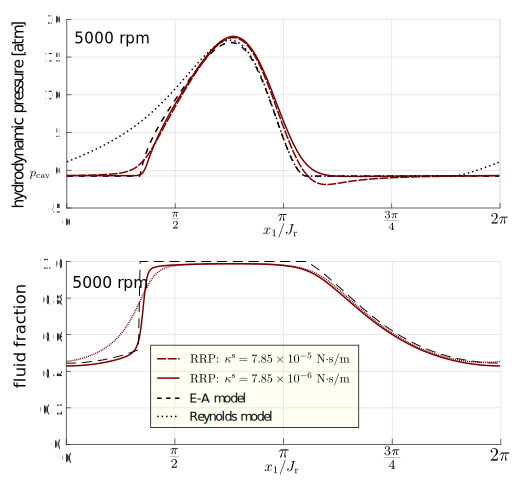
\includegraphics[scale=0.55]{comparison-ea-pressure.pdf}
	\end{figure}
\end{minipage}
\end{frame}  

%==============================================================
\begin{frame}
\frametitle{Numerical results: comparison with E-A}
\begin{minipage}{0.5\linewidth}\vspace*{1.0cm}
	\begin{figure}
		\includegraphics[scale=0.6]{journal_scheme_bw2.pdf}
	\end{figure}
\end{minipage}%
\hspace*{0.5cm}
\begin{minipage}{0.5\linewidth}
A comparison to look for the inertial terms relevance is made by solving the RRP model coupled with the Newton equation for the journal position $(X,Y)$. The journal is perturbed by applying a periodical force.\\

The journal's eccentricity reads $\varepsilon=\frac{\sqrt{X^2+Y^2}}{c}$. The force applied on the journal is set to
\begin{equation*}
\mathbf{W}^\textnormal{a}(t)=\mathbf{W}^{\textnormal{a},\textnormal{c}}+\mathbf{W}^{\textnormal{a},\textnormal{p}}(t)~.
\end{equation*}
\end{minipage}
\vspace*{-0.2cm}
\begin{figure}
	\centering 
	\def\svgwidth{\textwidth}	
	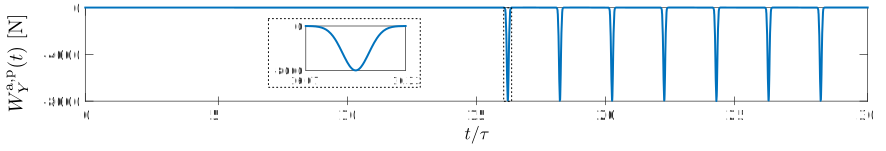
\includegraphics[scale=0.5]{WY_journal.pdf}
\end{figure}
\end{frame}  

%==============================================================
\begin{frame}\vspace*{0.5cm}
\frametitle{Numerical results: inertial terms relevance}
\begin{figure}
	\centering 
	\def\svgwidth{\textwidth}	
	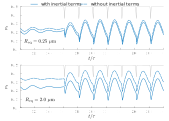
\includegraphics[scale=0.6]{ecc-journal_Req}
\end{figure}
\end{frame}  

%==============================================================
\begin{frame}\vspace*{0.5cm}
\frametitle{Numerical results: inertial terms relevance}
\begin{figure}\hspace*{-0.5cm}
	\centering 
	\def\svgwidth{\textwidth}	
	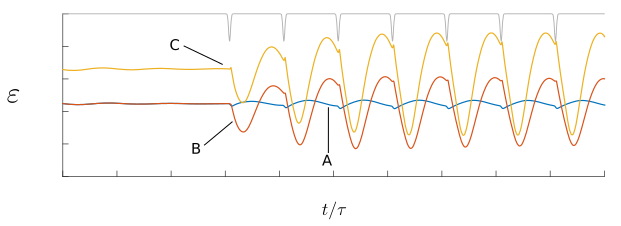
\includegraphics[scale=0.7]{ecc-journal-varying-Wa_strong}
\end{figure}
\begin{minipage}{.6\linewidth}
	The friction torque may be computed as
\begin{equation*}
\tau(t)=J_\textnormal{r}\int_\Omega\left( \frac{h(x_1,t)}{2}\parder{p}{x_1}+ \frac{\mu\left(R(x_1,t)\right){U}}{h(x_1,t)}\right)d\Omega,
\end{equation*}
\end{minipage}%
\begin{minipage}{.5\linewidth}
\begin{table}[h]
	\begin{center}
		\begin{tabular}{lccc}
			\toprule 
			& A & B & C \\
			\midrule
			$\left|\frac{\bar{\tau}_\textnormal{+i}-\bar{\tau}_\textnormal{-i}}{\bar{\tau}_\textnormal{+i}}\right|$ & 0.2\%& 1.2\% & 3.2\% \\
			\midrule
		\end{tabular} 
	\end{center}
\end{table}
\end{minipage}
\end{frame}  

%==============================================================
\begin{frame}
\frametitle{Conclusions}
\begin{itemize}
\item By means of a mass-conserving cavitation model, it has been observed that the shape of the pressurized regions in a lubricated device is influenced by the boundary conditions on pressure. This effect cannot be neglected when looking for accurate results on tribological measures prediction, like friction and minimum-film-thickness.
\item This kind of modeling can be useful to predict blow-by inception from high pressure gradients. This would to look for optimal geometries in the sense of \emph{sealing capacity}.

\end{itemize}
\end{frame}  

%==============================================================
\begin{frame}
\frametitle{Conclusions}
\begin{itemize}
	\item The well-posedness of the RRP coupling (disregarding bubbles convection) has been addressed by means of standard mathematical tools.
	\item Robust numerical methods for the RRP coupling in both the cases with and without inertial terms have been developed.
	
	\item For fast bubbles' dynamics (small $\kappa^s$) the Elrod-Adams model gives results similar to those of the RRP model. This is remarkable considering that the former model is a phenomenological one.
	
	\item For a wide spectrum of parameters, the RRP without inertial terms seems to be a good approximation to the full model. However, for certain configurations the inertial terms effects are not negligible.
\end{itemize}
\end{frame}  

%==============================================================
\begin{frame}
\frametitle{Future work}
\vspace*{0.5cm}
\noindent\textbf{On the non-homogeneous boundary conditions for pressure}
\begin{enumerate}
	\item To propose dynamical models for the rupture boundary along the mass conserving condition allowing both the surfaces to be textured in the two-dimensional case.
\end{enumerate}

\noindent\textbf{On the Reynolds-Rayleigh-Plesset coupling}
\begin{enumerate}
	\item To consider the dynamics of polydisperse distributions of bubbles. The numerous works of Carrica's group (Carrica, 1999; Castro, 2016) for the dynamics of a two-phase flow around a ship indicate the multigroup approach as a promising framework for this task.% This would allow for more realistic modeling and the incorporation of bubbles interaction, like bubbles break-up or coalescence.
	
	\item To perform a mathematical analysis of the RRP coupling for $\mathbf{U}_b\neq 0$. Since in that case the r.h.s. of the evolution problem is unbounded, a more general theory is needed, like the Hille-Yosida Theorem (Pazy, 1983; Brezis, 2010).
\end{enumerate}
\end{frame}  

%==============================================================

\setcounter{showSlideNumbers}{0}
\begin{frame}[noframenumbering]
\frametitle{Thank you for your attention!}\centering


\end{frame}
%==============================================================

\end{document} 